\documentclass{article}

\usepackage{amsmath}
\usepackage{amssymb}
\usepackage{amsthm}
\usepackage[australian]{babel}
\usepackage{braket}
\usepackage[a4paper]{geometry}
\usepackage{tikz}

%\usetikzlibrary{external}
%\tikzexternalize[prefix=tikz/]

\newcommand{\defaulttensorsize}{10pt}
\newcommand{\tensorsize}{\defaulttensorsize}

\usetikzlibrary{patterns,patterns.meta}
\usetikzlibrary{shapes.geometric}
\usetikzlibrary{shapes.misc}
% Base style for tensors.
\tikzstyle{tensor}=[draw, inner sep=0, outer sep=0, minimum size=\tensorsize]
% Used for drawing gaps in the tensor network diagram.
\tikzstyle{notensor}=[inner sep=0, outer xsep=2pt, outer ysep=0, minimum size=\tensorsize]
% Style for A tensors: if a square-shaped node is desired instead, ‘circle’ can be removed here.
\tikzstyle{atensor}=[tensor, circle]
% Circular-style tensors, for regular matrices.
\tikzstyle{ctensor}=[tensor, circle]
% Diamond-style tensors, for diagonal matrices.
\tikzstyle{dtensor}=[tensor, diamond]
% MPO tensors.
\tikzstyle{wtensor}=[tensor]
% Left-/right-orthogonal tensors.
\tikzstyle{ltensor}=[tensor, rounded rectangle, rounded rectangle left arc=none]
\tikzstyle{rtensor}=[tensor, rounded rectangle, rounded rectangle right arc=none]
% Environment (E/F) tensors.
\tikzstyle{etensor}=[tensor, minimum height=(1cm/\defaulttensorsize*0.5*2+1)*\tensorsize]
% Wide tensors, e.g. multi-site operators: argument specifies how many sites wide.
\tikzstyle{widetensor}[2]=[tensor, minimum width=(1cm/\defaulttensorsize*0.75*(#1-1)+1)*\tensorsize]
% Diagonal striped pattern.
\newcommand{\stripesize}{4pt}
\pgfdeclarepatternformonly{stripes}{\pgfpointorigin}{\pgfpoint{\stripesize}{\stripesize}}{\pgfpoint{\stripesize}{\stripesize}}
{
    \pgfpathmoveto{\pgfpoint{0}{0}}
    \pgfpathlineto{\pgfpoint{\stripesize}{\stripesize}}
    \pgfpathlineto{\pgfpoint{\stripesize}{0.5*\stripesize}}
    \pgfpathlineto{\pgfpoint{0.5*\stripesize}{0}}
    \pgfpathclose%
    \pgfusepath{fill}
    \pgfpathmoveto{\pgfpoint{0}{0.5*\stripesize}}
    \pgfpathlineto{\pgfpoint{0}{\stripesize}}
    \pgfpathlineto{\pgfpoint{0.5*\stripesize}{\stripesize}}
    \pgfpathclose%
    \pgfusepath{fill}
}
\tikzstyle{striped}=[pattern=stripes, pattern color=lightgray]

\tikzstyle{tensornetwork}=[baseline=-0.25em, xscale=0.75, yscale=0.5,
                           % Default padding for labels.
                           every node/.style={inner sep=0, outer xsep=2pt, outer ysep=5pt, text depth=0pt},
                           % Add some padding around the picture.
                           execute at end picture={\path (current bounding box.south west) +(-2pt, 0) (current bounding box.north east) +(2pt, 0);}]

% Deprecated styles.
% Triangular-style tensors
%\tikzstyle{ltensor}=[tensor, isosceles triangle, shape border rotate=0, isosceles triangle apex angle=60]
%\tikzstyle{rtensor}=[tensor, isosceles triangle, shape border rotate=180, isosceles triangle apex angle=60]
% Drawing left-/right-orthogonal tensors as isosceles triangles results in an
% undesirable alignment, so we draw them as trapezia instead where one of the
% parallel edges has zero length.
% (For some reason, inner xsep=0pt produces an error, so we just use 0.001pt.)
%\tikzstyle{ltensor}=[tensor, trapezium, shape border rotate=270, trapezium stretches, minimum width=20pt/sqrt(3), minimum height=10pt, inner xsep=0.001pt, shape border rotate=270]
%\tikzstyle{rtensor}=[tensor, trapezium, shape border rotate=270, trapezium stretches, minimum width=20pt/sqrt(3), minimum height=10pt, inner xsep=0.001pt, shape border rotate=90]

\title{Ti\textit{k}Z tensor network diagrams}
\author{Jesse Osborne}

\begin{document}
\maketitle

\noindent
Finite MPS:
\begin{equation}
    \ket{\Psi} =
    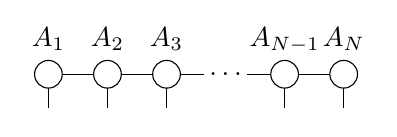
\begin{tikzpicture}[tensornetwork]
        \node[atensor, label=\(A_1\)]     (A1) at (1, 0) {};
        \node[atensor, label=\(A_2\)]     (A2) at (2, 0) {};
        \node[atensor, label=\(A_3\)]     (A3) at (3, 0) {};
        \node[notensor]                   (A4) at (4, 0) {\(\ldots\)};
        \node[atensor, label=\(A_{N-1}\)] (A5) at (5, 0) {};
        \node[atensor, label=\(A_N\)]     (A6) at (6, 0) {};
        \draw (A1.south) -- +(0, -0.5);
        \draw (A2.south) -- +(0, -0.5);
        \draw (A3.south) -- +(0, -0.5);
        \draw (A5.south) -- +(0, -0.5);
        \draw (A6.south) -- +(0, -0.5);
        \draw (A1) -- (A2) -- (A3) -- (A4) -- (A5) -- (A6);
    \end{tikzpicture}
    .
\end{equation}
Gauge transform:
\begin{equation}
    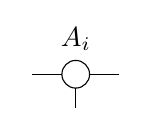
\begin{tikzpicture}[tensornetwork]
        \node[atensor, label=\(A_i\)] (A1) at (1, 0) {};
        \draw (A1.south) -- +(0, -0.5);
        \draw (A1.west) -- +(-0.5, 0);
        \draw (A1.east) -- +(0.5, 0);
    \end{tikzpicture}
    \rightarrow
    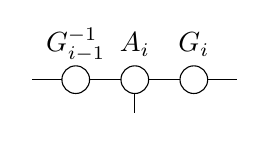
\begin{tikzpicture}[tensornetwork]
        \node[ctensor, label=\(G_{i-1}^{-1}\)] (G0inv) at (0, 0) {};
        \node[atensor, label=\(A_i\)] (A1) at (1, 0) {};
        \node[ctensor, label=\(G_i\)] (G1) at (2, 0) {};
        \draw (A1.south) -- +(0, -0.5);
        \draw (G0inv.west) -- +(-0.5, 0);
        \draw (G1.east) -- +(0.5, 0);
        \draw (G0inv) -- (A1) -- (G1);
    \end{tikzpicture}
    .
\end{equation}
Left-orthogonal form:
\begin{equation}
    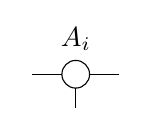
\begin{tikzpicture}[tensornetwork]
        \node[atensor, label=\(A_i\)] (A1) at (1, 0) {};
        \draw (A1.south) -- +(0, -0.5);
        \draw (A1.west) -- +(-0.5, 0);
        \draw (A1.east) -- +(0.5, 0);
    \end{tikzpicture}
    \rightarrow
    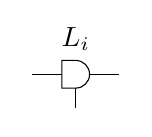
\begin{tikzpicture}[tensornetwork]
        \node[ltensor, label=\(L_i\)] (A1) at (1, 0) {};
        \draw (A1.south) -- +(0, -0.5);
        \draw (A1.west) -- +(-0.5, 0);
        \draw (A1.east) -- +(0.5, 0);
    \end{tikzpicture}
    ,
    \qquad
    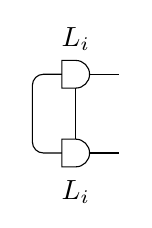
\begin{tikzpicture}[tensornetwork]
        \node[ltensor, label=\(L_i\)] (A1) at (1, 1) {};
        \node[ltensor, label=below:\(L_i\)] (A1conj) at (1, -1) {};
        \draw (A1.south) -- (A1conj.north);
        \draw[rounded corners] (A1.west) -- +(-0.5, 0) -- +(-0.5, -2) -- (A1conj.west);
        \draw (A1.east) -- +(0.5, 0);
        \draw (A1conj.east) -- +(0.5, 0);
    \end{tikzpicture}
    =
    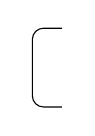
\begin{tikzpicture}[tensornetwork]
        \draw[rounded corners] (0, 1) -- +(-0.5, 0) -- +(-0.5, -2) -- +(0, -2);
    \end{tikzpicture}
    .
\end{equation}
Right-orthogonal form:
\begin{equation}
    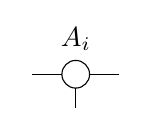
\begin{tikzpicture}[tensornetwork]
        \node[atensor, label=\(A_i\)] (A1) at (1, 0) {};
        \draw (A1.south) -- +(0, -0.5);
        \draw (A1.west) -- +(-0.5, 0);
        \draw (A1.east) -- +(0.5, 0);
    \end{tikzpicture}
    \rightarrow
    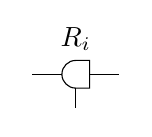
\begin{tikzpicture}[tensornetwork]
        \node[rtensor, label=\(R_i\)] (A1) at (1, 0) {};
        \draw (A1.south) -- +(0, -0.5);
        \draw (A1.west) -- +(-0.5, 0);
        \draw (A1.east) -- +(0.5, 0);
    \end{tikzpicture}
    ,
    \qquad
    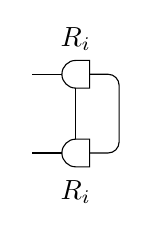
\begin{tikzpicture}[tensornetwork]
        \node[rtensor, label=\(R_i\)] (A1) at (1, 1) {};
        \node[rtensor, label=below:\(R_i\)] (A1conj) at (1, -1) {};
        \draw (A1.south) -- (A1conj.north);
        \draw[rounded corners] (A1.east) -- +(0.5, 0) -- +(0.5, -2) -- (A1conj.east);
        \draw (A1.west) -- +(-0.5, 0);
        \draw (A1conj.west) -- +(-0.5, 0);
    \end{tikzpicture}
    =
    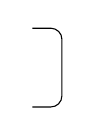
\begin{tikzpicture}[tensornetwork]
        \draw[rounded corners] (0, 1) -- +(0.5, 0) -- +(0.5, -2) -- +(0, -2);
    \end{tikzpicture}
    .
\end{equation}
SVD:
\begin{equation}
    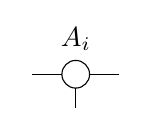
\begin{tikzpicture}[tensornetwork]
        \node[atensor, label=\(A_i\)] (A1) at (1, 0) {};
        \draw (A1.south) -- +(0, -0.5);
        \draw (A1.west) -- +(-0.5, 0);
        \draw (A1.east) -- +(0.5, 0);
    \end{tikzpicture}
    =
    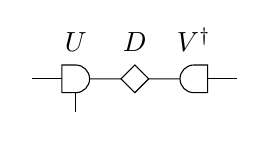
\begin{tikzpicture}[tensornetwork]
        \node[ltensor, label=\(U\)] (A1) at (0, 0) {};
        \node[dtensor, label=\(D\)] (D) at (1, 0) {};
        \node[rtensor, label=\(V^\dag\)] (Vdag) at (2, 0) {};
        \draw (A1.south) -- +(0, -0.5);
        \draw (A1.west) -- +(-0.5, 0);
        \draw (Vdag.east) -- +(0.5, 0);
        \draw (A1) -- (D) -- (Vdag);
    \end{tikzpicture}
    .
\end{equation}
Mixed-canonical form:
\begin{equation}
    \ket{\Psi} =
    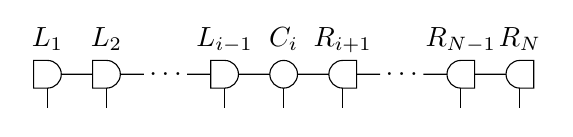
\begin{tikzpicture}[tensornetwork]
        \node[ltensor, label=\(L_1\)]     (A1) at (1, 0) {};
        \node[ltensor, label=\(L_2\)]     (A2) at (2, 0) {};
        \node[notensor]                   (A3) at (3, 0) {\(\ldots\)};
        \node[ltensor, label=\(L_{i-1}\)] (A4) at (4, 0) {};
        \node[atensor, label=\(C_i\)]     (A5) at (5, 0) {};
        \node[rtensor, label=\(R_{i+1}\)] (A6) at (6, 0) {};
        \node[notensor]                   (A7) at (7, 0) {\(\ldots\)};
        \node[rtensor, label=\(R_{N-1}\)] (A8) at (8, 0) {};
        \node[rtensor, label=\(R_N\)]     (A9) at (9, 0) {};
        \draw (A1.south) -- +(0, -0.5);
        \draw (A2.south) -- +(0, -0.5);
        \draw (A4.south) -- +(0, -0.5);
        \draw (A5.south) -- +(0, -0.5);
        \draw (A6.south) -- +(0, -0.5);
        \draw (A8.south) -- +(0, -0.5);
        \draw (A9.south) -- +(0, -0.5);
        \draw (A1) -- (A2) -- (A3) -- (A4) -- (A5) -- (A6) -- (A7) -- (A8) -- (A9);
    \end{tikzpicture}
    .
\end{equation}
\begin{equation}
    \ket{\Psi} =
    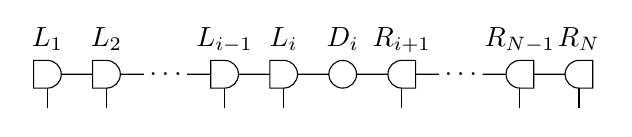
\begin{tikzpicture}[tensornetwork]
        \node[ltensor, label=\(L_1\)]     (A1) at (1, 0) {};
        \node[ltensor, label=\(L_2\)]     (A2) at (2, 0) {};
        \node[notensor]                   (A3) at (3, 0) {\(\ldots\)};
        \node[ltensor, label=\(L_{i-1}\)] (A4) at (4, 0) {};
        \node[ltensor, label=\(L_{i}\)]   (A5) at (5, 0) {};
        \node[ctensor, label=\(D_i\)]     (D)  at (6, 0) {};
        \node[rtensor, label=\(R_{i+1}\)] (A6) at (7, 0) {};
        \node[notensor]                   (A7) at (8, 0) {\(\ldots\)};
        \node[rtensor, label=\(R_{N-1}\)] (A8) at (9, 0) {};
        \node[rtensor, label=\(R_N\)]     (A9) at (10, 0) {};
        \draw (A1.south) -- +(0, -0.5);
        \draw (A2.south) -- +(0, -0.5);
        \draw (A4.south) -- +(0, -0.5);
        \draw (A5.south) -- +(0, -0.5);
        \draw (A6.south) -- +(0, -0.5);
        \draw (A8.south) -- +(0, -0.5);
        \draw (A9.south) -- +(0, -0.5);
        \draw (A1) -- (A2) -- (A3) -- (A4) -- (A5) -- (D) -- (A6) -- (A7) -- (A8) -- (A9);
    \end{tikzpicture}
    .
\end{equation}
Unitary gauge transformation:
\begin{equation}
    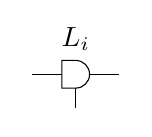
\begin{tikzpicture}[tensornetwork]
        \node[ltensor, label=\(L_i\)] (A1) at (1, 0) {};
        \draw (A1.south) -- +(0, -0.5);
        \draw (A1.west) -- +(-0.5, 0);
        \draw (A1.east) -- +(0.5, 0);
    \end{tikzpicture}
    \rightarrow
    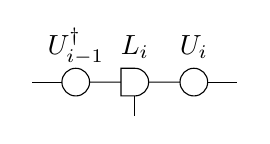
\begin{tikzpicture}[tensornetwork]
        \node[ctensor, label=\(U_{i-1}^\dag\)] (G0inv) at (0, 0) {};
        \node[ltensor, label=\(L_i\)] (A1) at (1, 0) {};
        \node[ctensor, label=\(U_i\)] (G1) at (2, 0) {};
        \draw (A1.south) -- +(0, -0.5);
        \draw (G0inv.west) -- +(-0.5, 0);
        \draw (G1.east) -- +(0.5, 0);
        \draw (G0inv) -- (A1) -- (G1);
    \end{tikzpicture}
    .
\end{equation}
Expectation value:
\begin{equation}
    \braket{\Psi|O_i|\Psi} =
    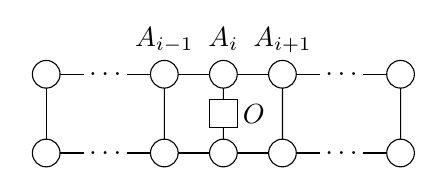
\begin{tikzpicture}[tensornetwork]
        \node[atensor]                    (A1) at (1, 1) {};
        \node[notensor]                   (A2) at (2, 1) {\(\ldots\)};
        \node[atensor, label=\(A_{i-1}\)] (A3) at (3, 1) {};
        \node[atensor, label=\(A_i\)]     (A4) at (4, 1) {};
        \node[atensor, label=\(A_{i+1}\)] (A5) at (5, 1) {};
        \node[notensor]                   (A6) at (6, 1) {\(\ldots\)};
        \node[atensor]                    (A7) at (7, 1) {};
        \node[atensor]                    (A1conj) at (1, -1) {};
        \node[notensor]                   (A2conj) at (2, -1) {\(\ldots\)};
        \node[atensor]                    (A3conj) at (3, -1) {};
        \node[atensor]                    (A4conj) at (4, -1) {};
        \node[atensor]                    (A5conj) at (5, -1) {};
        \node[notensor]                   (A6conj) at (6, -1) {\(\ldots\)};
        \node[atensor]                    (A7conj) at (7, -1) {};
        \node[wtensor, label={right, text depth=}:\(O\)] (O) at (4, 0) {};
        \draw (A1) -- (A1conj);
        \draw (A3) -- (A3conj);
        \draw (A4) -- (O) -- (A4conj);
        \draw (A5) -- (A5conj);
        \draw (A7) -- (A7conj);
        \draw (A1) -- (A2) -- (A3) -- (A4) -- (A5) -- (A6) -- (A7);
        \draw (A1conj) -- (A2conj) -- (A3conj) -- (A4conj) -- (A5conj) -- (A6conj) -- (A7conj);
    \end{tikzpicture}
    .
\end{equation}
\begin{equation}
    \braket{\Psi|O_i|\Psi} =
    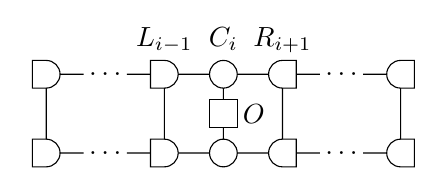
\begin{tikzpicture}[tensornetwork]
        \node[ltensor]                    (A1) at (1, 1) {};
        \node[notensor]                   (A2) at (2, 1) {\(\ldots\)};
        \node[ltensor, label=\(L_{i-1}\)] (A3) at (3, 1) {};
        \node[atensor, label=\(C_i\)]     (A4) at (4, 1) {};
        \node[rtensor, label=\(R_{i+1}\)] (A5) at (5, 1) {};
        \node[notensor]                   (A6) at (6, 1) {\(\ldots\)};
        \node[rtensor]                    (A7) at (7, 1) {};
        \node[ltensor]                    (A1conj) at (1, -1) {};
        \node[notensor]                   (A2conj) at (2, -1) {\(\ldots\)};
        \node[ltensor]                    (A3conj) at (3, -1) {};
        \node[atensor]                    (A4conj) at (4, -1) {};
        \node[rtensor]                    (A5conj) at (5, -1) {};
        \node[notensor]                   (A6conj) at (6, -1) {\(\ldots\)};
        \node[rtensor]                    (A7conj) at (7, -1) {};
        \node[wtensor, label={right, text depth=}:\(O\)] (O) at (4, 0) {};
        \draw (A1) -- (A1conj);
        \draw (A3) -- (A3conj);
        \draw (A4) -- (O) -- (A4conj);
        \draw (A5) -- (A5conj);
        \draw (A7) -- (A7conj);
        \draw (A1) -- (A2) -- (A3) -- (A4) -- (A5) -- (A6) -- (A7);
        \draw (A1conj) -- (A2conj) -- (A3conj) -- (A4conj) -- (A5conj) -- (A6conj) -- (A7conj);
    \end{tikzpicture}
    =
    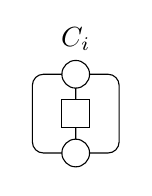
\begin{tikzpicture}[tensornetwork]
        \node[atensor, label=\(C_i\)] (A4) at (4, 1) {};
        \node[atensor]                (A4conj) at (4, -1) {};
        \node[wtensor]                (O) at (4, 0) {};
        \draw (A4) -- (O) -- (A4conj);
        \draw[rounded corners] (A4.west) -- +(-0.5, 0) -- +(-0.5, -2) -- (A4conj.west);
        \draw[rounded corners] (A4.east) -- +(0.5, 0) -- +(0.5, -2) -- (A4conj.east);
    \end{tikzpicture}
    .
\end{equation}
Multi-site expectation value:
\begin{equation}
    \braket{\Psi|O|\Psi} =
    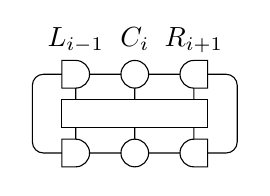
\begin{tikzpicture}[tensornetwork]
        \node[ltensor, label=\(L_{i-1}\)]  (A3) at (3, 1) {};
        \node[atensor, label=\(C_i\)]      (A4) at (4, 1) {};
        \node[rtensor, label=\(R_{i+1}\)]  (A5) at (5, 1) {};
        \node[ltensor]                     (A3conj) at (3, -1) {};
        \node[atensor]                     (A4conj) at (4, -1) {};
        \node[rtensor]                     (A5conj) at (5, -1) {};
        \node[widetensor=3]                (O) at (4, 0) {};
        \draw (A3) -- (O.north -| A3);
        \draw (A3conj) -- (O.south -| A3conj);
        \draw (A4) -- (O.north -| A4);
        \draw (A4conj) -- (O.south -| A4conj);
        \draw (A5) -- (O.north -| A5);
        \draw (A5conj) -- (O.south -| A5conj);
        \draw (A3) -- (A4) -- (A5);
        \draw (A3conj) -- (A4conj) -- (A5conj);
        \draw[rounded corners] (A3.west) -- +(-0.5, 0) -- +(-0.5, -2) -- (A3conj.west);
        \draw[rounded corners] (A5.east) -- +(0.5, 0) -- +(0.5, -2) -- (A5conj.east);
    \end{tikzpicture}
    .
\end{equation}
MPO:
\begin{equation}
    \begin{tikzpicture}[tensornetwork]
        \node[widetensor=3] (O) at (4, 0) {};
        \coordinate (A3) at (3, 0.5) {};
        \coordinate (A4) at (4, 0.5) {};
        \coordinate (A5) at (5, 0.5) {};
        \draw (O.north -| A3) -- +(0, 0.5);
        \draw (O.north -| A4) -- +(0, 0.5);
        \draw (O.north -| A5) -- +(0, 0.5);
        \draw (O.south -| A3) -- +(0, -0.5);
        \draw (O.south -| A4) -- +(0, -0.5);
        \draw (O.south -| A5) -- +(0, -0.5);
    \end{tikzpicture}
    =
    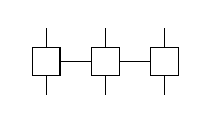
\begin{tikzpicture}[tensornetwork]
        \node[wtensor] (W3) at (3, 0) {};
        \node[wtensor] (W4) at (4, 0) {};
        \node[wtensor] (W5) at (5, 0) {};
        \draw (W3.north) -- +(0, 0.5);
        \draw (W4.north) -- +(0, 0.5);
        \draw (W5.north) -- +(0, 0.5);
        \draw (W3.south) -- +(0, -0.5);
        \draw (W4.south) -- +(0, -0.5);
        \draw (W5.south) -- +(0, -0.5);
        \draw (W3) -- (W4) -- (W5);
    \end{tikzpicture}
    .
\end{equation}
MPO expectation value:
\begin{equation}
    \braket{\Psi|H|\Psi} =
    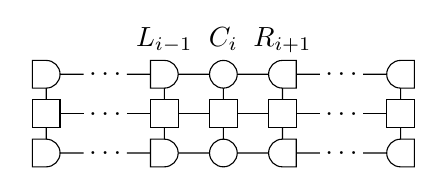
\begin{tikzpicture}[tensornetwork]
        \node[ltensor]                    (A1) at (1, 1) {};
        \node[notensor]                   (A2) at (2, 1) {\(\ldots\)};
        \node[ltensor, label=\(L_{i-1}\)] (A3) at (3, 1) {};
        \node[atensor, label=\(C_i\)]     (A4) at (4, 1) {};
        \node[rtensor, label=\(R_{i+1}\)] (A5) at (5, 1) {};
        \node[notensor]                   (A6) at (6, 1) {\(\ldots\)};
        \node[rtensor]                    (A7) at (7, 1) {};
        \node[ltensor]                    (A1conj) at (1, -1) {};
        \node[notensor]                   (A2conj) at (2, -1) {\(\ldots\)};
        \node[ltensor]                    (A3conj) at (3, -1) {};
        \node[atensor]                    (A4conj) at (4, -1) {};
        \node[rtensor]                    (A5conj) at (5, -1) {};
        \node[notensor]                   (A6conj) at (6, -1) {\(\ldots\)};
        \node[rtensor]                    (A7conj) at (7, -1) {};
        \node[wtensor]                    (W1) at (1, 0) {};
        \node[notensor]                   (W2) at (2, 0) {\(\ldots\)};
        \node[wtensor]                    (W3) at (3, 0) {};
        \node[wtensor]                    (W4) at (4, 0) {};
        \node[wtensor]                    (W5) at (5, 0) {};
        \node[notensor]                   (W6) at (6, 0) {\(\ldots\)};
        \node[wtensor]                    (W7) at (7, 0) {};
        \draw (A1) -- (W1) -- (A1conj);
        \draw (A3) -- (W3) -- (A3conj);
        \draw (A4) -- (W4) -- (A4conj);
        \draw (A5) -- (W5) -- (A5conj);
        \draw (A7) -- (W7) -- (A7conj);
        \draw (A1) -- (A2) -- (A3) -- (A4) -- (A5) -- (A6) -- (A7);
        \draw (W1) -- (W2) -- (W3) -- (W4) -- (W5) -- (W6) -- (W7);
        \draw (A1conj) -- (A2conj) -- (A3conj) -- (A4conj) -- (A5conj) -- (A6conj) -- (A7conj);
    \end{tikzpicture}
    =
    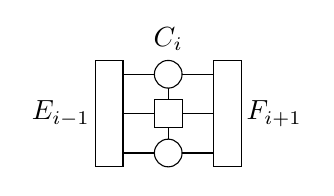
\begin{tikzpicture}[tensornetwork]
        \node[atensor, label=\(C_i\)]           (A1) at (0, 1) {};
        \node[atensor]                          (A1conj) at (0, -1) {};
        \node[wtensor]                          (W4) at (0, 0) {};
        \node[etensor, label={left, text depth=}:\(E_{i-1}\)]  (E) at (-1, 0) {};
        \node[etensor, label={right, text depth=}:\(F_{i+1}\)] (F) at (1, 0) {};
        \draw (A1) -- (W4) -- (A1conj);
        \draw (E) -- (W4) -- (F);
        \draw (A1) -- (E.east |- A1);
        \draw (A1conj) -- (E.east |- A1conj);
        \draw (A1) -- (F.west |- A1);
        \draw (A1conj) -- (F.west |- A1conj);
    \end{tikzpicture}
    =
    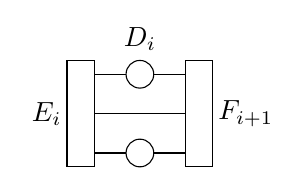
\begin{tikzpicture}[tensornetwork]
        \node[ctensor, label=\(D_i\)]           (A1) at (0, 1) {};
        \node[ctensor]                          (A1conj) at (0, -1) {};
        \node[etensor, label={left, text depth=}:\(E_i\)]      (E) at (-1, 0) {};
        \node[etensor, label={right, text depth=}:\(F_{i+1}\)] (F) at (1, 0) {};
        \draw (E) -- (F);
        \draw (A1) -- (E.east |- A1);
        \draw (A1conj) -- (E.east |- A1conj);
        \draw (A1) -- (F.west |- A1);
        \draw (A1conj) -- (F.west |- A1conj);
    \end{tikzpicture}
    .
\end{equation}
Environment tensors:
\begin{equation}
    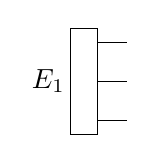
\begin{tikzpicture}[tensornetwork]
        \coordinate (A1) at (0, 1) {};
        \coordinate (A1conj) at (0, -1) {};
        \node[etensor, label={left, text depth=}:\(E_1\)] (E) at (-1, 0) {};
        \draw (E.east) -- +(0.5, 0);
        \draw (E.east |- A1) -- +(0.5, 0);
        \draw (E.east |- A1conj) -- +(0.5, 0);
    \end{tikzpicture}
    \equiv
    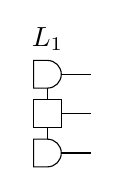
\begin{tikzpicture}[tensornetwork]
        \node[ltensor, label=\(L_1\)] (A1) at (0, 1) {};
        \node[ltensor]                (A1conj) at (0, -1) {};
        \node[wtensor]                (W1) at (0, 0) {};
        \draw (A1.east) -- +(0.5, 0);
        \draw (A1conj.east) -- +(0.5, 0);
        \draw (W1.east) -- +(0.5, 0);
        \draw (A1) -- (W1) -- (A1conj);
    \end{tikzpicture}
    ,\qquad
    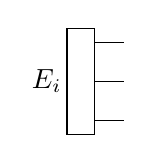
\begin{tikzpicture}[tensornetwork]
        \coordinate (A1) at (0, 1) {};
        \coordinate (A1conj) at (0, -1) {};
        \node[etensor, label={left, text depth=}:\(E_i\)] (E) at (-1, 0) {};
        \draw (E.east) -- +(0.5, 0);
        \draw (E.east |- A1) -- +(0.5, 0);
        \draw (E.east |- A1conj) -- +(0.5, 0);
    \end{tikzpicture}
    \equiv
    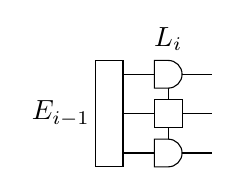
\begin{tikzpicture}[tensornetwork]
        \node[ltensor, label=\(L_i\)]          (A1) at (0, 1) {};
        \node[ltensor]                         (A1conj) at (0, -1) {};
        \node[wtensor]                         (W1) at (0, 0) {};
        \node[etensor, label={left, text depth=}:\(E_{i-1}\)] (E) at (-1, 0) {};
        \draw (A1.east) -- +(0.5, 0);
        \draw (A1conj.east) -- +(0.5, 0);
        \draw (W1.east) -- +(0.5, 0);
        \draw (A1) -- (W1) -- (A1conj);
        \draw (E) -- (W1);
        \draw (A1) -- (E.east |- A1);
        \draw (A1conj) -- (E.east |- A1conj);
    \end{tikzpicture}
    .
\end{equation}
\begin{equation}
    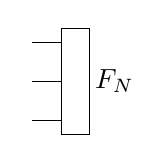
\begin{tikzpicture}[tensornetwork]
        \coordinate (A1) at (0, 1) {};
        \coordinate (A1conj) at (0, -1) {};
        \node[etensor, label={right, text depth=}:\(F_N\)] (F) at (1, 0) {};
        \draw (F.west) -- +(-0.5, 0);
        \draw (F.west|- A1) -- +(-0.5, 0);
        \draw (F.west |- A1conj) -- +(-0.5, 0);
    \end{tikzpicture}
    \equiv
    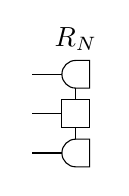
\begin{tikzpicture}[tensornetwork]
        \node[rtensor, label=\(R_N\)] (A1) at (0, 1) {};
        \node[rtensor]                (A1conj) at (0, -1) {};
        \node[wtensor]                (W1) at (0, 0) {};
        \draw (A1.west) -- +(-0.5, 0);
        \draw (A1conj.west) -- +(-0.5, 0);
        \draw (W1.west) -- +(-0.5, 0);
        \draw (A1) -- (W1) -- (A1conj);
    \end{tikzpicture}
    ,\qquad
    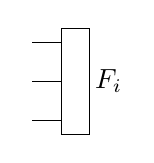
\begin{tikzpicture}[tensornetwork]
        \coordinate (A1) at (0, 1) {};
        \coordinate (A1conj) at (0, -1) {};
        \node[etensor, label={right, text depth=}:\(F_i\)] (F) at (1, 0) {};
        \draw (F.west) -- +(-0.5, 0);
        \draw (F.west|- A1) -- +(-0.5, 0);
        \draw (F.west |- A1conj) -- +(-0.5, 0);
    \end{tikzpicture}
    \equiv
    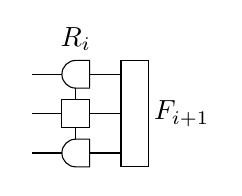
\begin{tikzpicture}[tensornetwork]
        \node[rtensor, label=\(R_i\)]           (A1) at (0, 1) {};
        \node[rtensor]                          (A1conj) at (0, -1) {};
        \node[wtensor]                          (W1) at (0, 0) {};
        \node[etensor, label={right, text depth=}:\(F_{i+1}\)] (F) at (1, 0) {};
        \draw (A1.west) -- +(-0.5, 0);
        \draw (A1conj.west) -- +(-0.5, 0);
        \draw (W1.west) -- +(-0.5, 0);
        \draw (A1) -- (W1) -- (A1conj);
        \draw (W1) -- (F);
        \draw (A1) -- (F.west |- A1);
        \draw (A1conj) -- (F.west |- A1conj);
    \end{tikzpicture}
    .
\end{equation}
iMPS:
\begin{equation}
    \ket{\Psi} =
    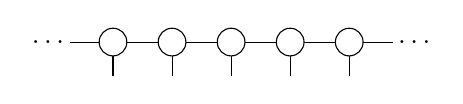
\begin{tikzpicture}[tensornetwork]
        \node[atensor] (A1) at (1, 0) {};
        \node[atensor] (A2) at (2, 0) {};
        \node[atensor] (A3) at (3, 0) {};
        \node[atensor] (A4) at (4, 0) {};
        \node[atensor] (A5) at (5, 0) {};
        \draw (A1.south) -- +(0, -0.5);
        \draw (A2.south) -- +(0, -0.5);
        \draw (A3.south) -- +(0, -0.5);
        \draw (A4.south) -- +(0, -0.5);
        \draw (A5.south) -- +(0, -0.5);
        \draw (A1) -- (A2) -- (A3) -- (A4) -- (A5);
        \draw (A1.west) -- +(-0.5, 0) node[left] {\(\ldots\)};
        \draw (A5.east) -- +(0.5, 0) node[right] {\(\ldots\)};
    \end{tikzpicture}
    .
\end{equation}
Transfer matrix:
\begin{equation}
    T =
    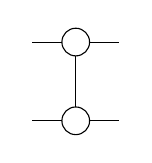
\begin{tikzpicture}[tensornetwork]
        \node[atensor] (A1) at (0, 1) {};
        \node[atensor] (A1conj) at (0, -1) {};
        \draw (A1) -- (A1conj);
        \draw (A1.west) -- +(-0.5, 0);
        \draw (A1.east) -- +(0.5, 0);
        \draw (A1conj.west) -- +(-0.5, 0);
        \draw (A1conj.east) -- +(0.5, 0);
    \end{tikzpicture}
    .
\end{equation}
MPS norm:
\begin{equation}
    \braket{\Psi|\Psi} =
    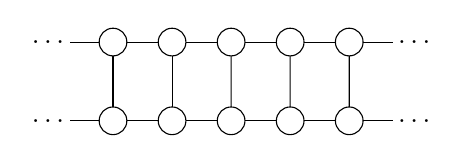
\begin{tikzpicture}[tensornetwork]
        \node[atensor] (A1) at (1, 1) {};
        \node[atensor] (A2) at (2, 1) {};
        \node[atensor] (A3) at (3, 1) {};
        \node[atensor] (A4) at (4, 1) {};
        \node[atensor] (A5) at (5, 1) {};
        \node[atensor] (A1conj) at (1, -1) {};
        \node[atensor] (A2conj) at (2, -1) {};
        \node[atensor] (A3conj) at (3, -1) {};
        \node[atensor] (A4conj) at (4, -1) {};
        \node[atensor] (A5conj) at (5, -1) {};
        \draw (A1) -- (A1conj);
        \draw (A2) -- (A2conj);
        \draw (A3) -- (A3conj);
        \draw (A4) -- (A4conj);
        \draw (A5) -- (A5conj);
        \draw (A1) -- (A2) -- (A3) -- (A4) -- (A5);
        \draw (A1conj) -- (A2conj) -- (A3conj) -- (A4conj) -- (A5conj);
        \draw (A1.west) -- +(-0.5, 0) node[left] {\(\ldots\)};
        \draw (A5.east) -- +(0.5, 0) node[right] {\(\ldots\)};
        \draw (A1conj.west) -- +(-0.5, 0) node[left] {\(\ldots\)};
        \draw (A5conj.east) -- +(0.5, 0) node[right] {\(\ldots\)};
    \end{tikzpicture}
    .
\end{equation}
Left-orthogonal form:
\begin{equation}
    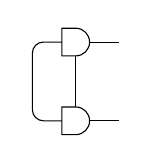
\begin{tikzpicture}[tensornetwork]
        \node[ltensor] (A1) at (0, 1) {};
        \node[ltensor] (A1conj) at (0, -1) {};
        \draw (A1.south) -- (A1conj.north);
        \draw[rounded corners] (A1.west) -- +(-0.5, 0) -- +(-0.5, -2) -- (A1conj.west);
        \draw (A1.east) -- +(0.5, 0);
        \draw (A1conj.east) -- +(0.5, 0);
    \end{tikzpicture}
    =
    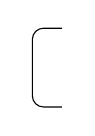
\begin{tikzpicture}[tensornetwork]
        \draw[rounded corners] (0, 1) -- +(-0.5, 0) -- +(-0.5, -2) -- +(0, -2);
    \end{tikzpicture}
    ,
    \qquad
    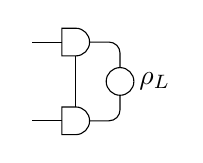
\begin{tikzpicture}[tensornetwork]
        \node[ltensor] (A1) at (0, 1) {};
        \node[ltensor] (A1conj) at (0, -1) {};
        \node[ctensor, label={right, text depth=}:\(\rho_L\)] (rho) at (0.75, 0) {};
        \draw (A1.south) -- (A1conj.north);
        \draw[rounded corners] (A1.east) -- (A1.east -| rho.north) -- (rho) -- (rho.south |- A1conj.east) -- (A1conj.east);
        \draw (A1.west) -- +(-0.5, 0);
        \draw (A1conj.west) -- +(-0.5, 0);
    \end{tikzpicture}
    =
    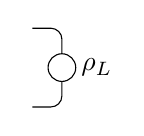
\begin{tikzpicture}[tensornetwork]
        \coordinate (A1) at (0, 1) {};
        \coordinate (A1conj) at (0, -1) {};
        \node[ctensor, label={right, text depth=}:\(\rho_L\)] (rho) at (0.75, 0) {};
        \draw[rounded corners] (rho.north) -- (rho.north |- A1.east) -- +(-0.5, 0);
        \draw[rounded corners] (rho.south) -- (rho.south |- A1conj.east) -- +(-0.5, 0);
    \end{tikzpicture}
    .
\end{equation}
Right-orthogonal form:
\begin{equation}
    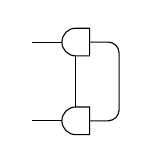
\begin{tikzpicture}[tensornetwork]
        \node[rtensor] (A1) at (0, 1) {};
        \node[rtensor] (A1conj) at (0, -1) {};
        \draw (A1.south) -- (A1conj.north);
        \draw[rounded corners] (A1.east) -- +(0.5, 0) -- +(0.5, -2) -- (A1conj.east);
        \draw (A1.west) -- +(-0.5, 0);
        \draw (A1conj.west) -- +(-0.5, 0);
    \end{tikzpicture}
    =
    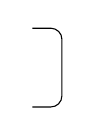
\begin{tikzpicture}[tensornetwork]
        \draw[rounded corners] (0, 1) -- +(0.5, 0) -- +(0.5, -2) -- +(0, -2);
    \end{tikzpicture}
    ,
    \qquad
    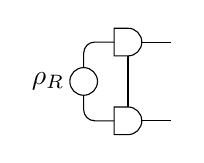
\begin{tikzpicture}[tensornetwork]
        \node[ltensor] (A1) at (0, 1) {};
        \node[ltensor] (A1conj) at (0, -1) {};
        \node[ctensor, label={left, text depth=}:\(\rho_R\)] (rho) at (-0.75, 0) {};
        \draw (A1.south) -- (A1conj.north);
        \draw[rounded corners] (A1.west) -- (A1.west -| rho.north) -- (rho) -- (rho.south |- A1conj.west) -- (A1conj.west);
        \draw (A1.east) -- +(0.5, 0);
        \draw (A1conj.east) -- +(0.5, 0);
    \end{tikzpicture}
    =
    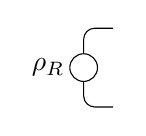
\begin{tikzpicture}[tensornetwork]
        \coordinate (A1) at (0, 1) {};
        \coordinate (A1conj) at (0, -1) {};
        \node[ctensor, label={left, text depth=}:\(\rho_R\)] (rho) at (-0.75, 0) {};
        \draw[rounded corners] (rho.north) -- (rho.north |- A1.west) -- +(0.5, 0);
        \draw[rounded corners] (rho.south) -- (rho.south |- A1conj.west) -- +(0.5, 0);
    \end{tikzpicture}
    .
\end{equation}
Mixed-canonical form:
\begin{align}
    \ket{\Psi} &=
    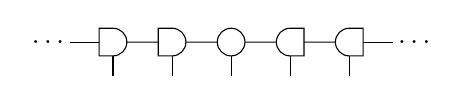
\begin{tikzpicture}[tensornetwork]
        \node[ltensor] (A1) at (1, 0) {};
        \node[ltensor] (A2) at (2, 0) {};
        \node[atensor] (A3) at (3, 0) {};
        \node[rtensor] (A4) at (4, 0) {};
        \node[rtensor] (A5) at (5, 0) {};
        \draw (A1.south) -- +(0, -0.5);
        \draw (A2.south) -- +(0, -0.5);
        \draw (A3.south) -- +(0, -0.5);
        \draw (A4.south) -- +(0, -0.5);
        \draw (A5.south) -- +(0, -0.5);
        \draw (A1) -- (A2) -- (A3) -- (A4) -- (A5);
        \draw (A1.west) -- +(-0.5, 0) node[left] {\(\ldots\)};
        \draw (A5.east) -- +(0.5, 0) node[right] {\(\ldots\)};
    \end{tikzpicture}
    \\
    &=
    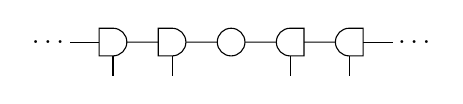
\begin{tikzpicture}[tensornetwork]
        \node[ltensor] (A1) at (1, 0) {};
        \node[ltensor] (A2) at (2, 0) {};
        \node[ctensor] (A3) at (3, 0) {};
        \node[rtensor] (A4) at (4, 0) {};
        \node[rtensor] (A5) at (5, 0) {};
        \draw (A1.south) -- +(0, -0.5);
        \draw (A2.south) -- +(0, -0.5);
        \draw (A4.south) -- +(0, -0.5);
        \draw (A5.south) -- +(0, -0.5);
        \draw (A1) -- (A2) -- (A3) -- (A4) -- (A5);
        \draw (A1.west) -- +(-0.5, 0) node[left] {\(\ldots\)};
        \draw (A5.east) -- +(0.5, 0) node[right] {\(\ldots\)};
    \end{tikzpicture}
    .
\end{align}
iMPS expectation value:
\begin{equation}
    \braket{\Psi|O_i|\Psi} =
    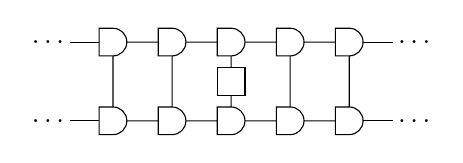
\begin{tikzpicture}[tensornetwork]
        \node[ltensor] (A1) at (1, 1) {};
        \node[ltensor] (A2) at (2, 1) {};
        \node[ltensor] (A3) at (3, 1) {};
        \node[ltensor] (A4) at (4, 1) {};
        \node[ltensor] (A5) at (5, 1) {};
        \node[ltensor] (A1conj) at (1, -1) {};
        \node[ltensor] (A2conj) at (2, -1) {};
        \node[ltensor] (A3conj) at (3, -1) {};
        \node[ltensor] (A4conj) at (4, -1) {};
        \node[ltensor] (A5conj) at (5, -1) {};
        \node[wtensor] (O) at (3, 0) {};
        \draw (A1) -- (A1conj);
        \draw (A2) -- (A2conj);
        \draw (A3) -- (O) -- (A3conj);
        \draw (A4) -- (A4conj);
        \draw (A5) -- (A5conj);
        \draw (A1) -- (A2) -- (A3) -- (A4) -- (A5);
        \draw (A1conj) -- (A2conj) -- (A3conj) -- (A4conj) -- (A5conj);
        \draw (A1.west) -- +(-0.5, 0) node[left] {\(\ldots\)};
        \draw (A5.east) -- +(0.5, 0) node[right] {\(\ldots\)};
        \draw (A1conj.west) -- +(-0.5, 0) node[left] {\(\ldots\)};
        \draw (A5conj.east) -- +(0.5, 0) node[right] {\(\ldots\)};
    \end{tikzpicture}
    =
    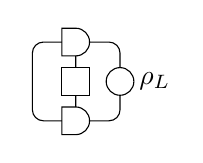
\begin{tikzpicture}[tensornetwork]
        \node[ltensor] (A3) at (3, 1) {};
        \node[ltensor] (A3conj) at (3, -1) {};
        \node[wtensor] (O) at (3, 0) {};
        \node[ctensor, label={right, text depth=}:\(\rho_L\)] (rho) at (3.75, 0) {};
        \draw (A3) -- (O) -- (A3conj);
        \draw[rounded corners] (A3.west) -- +(-0.5, 0) -- +(-0.5, -2) -- (A3conj.west);
        \draw[rounded corners] (A3.east) -- (A3.east -| rho.north) -- (rho) -- (rho.south |- A3conj.east) -- (A3conj.east);
    \end{tikzpicture}
    .
\end{equation}
\begin{equation}
    \braket{\Psi|O_i|\Psi} =
    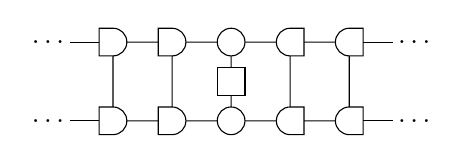
\begin{tikzpicture}[tensornetwork]
        \node[ltensor] (A1) at (1, 1) {};
        \node[ltensor] (A2) at (2, 1) {};
        \node[atensor] (A3) at (3, 1) {};
        \node[rtensor] (A4) at (4, 1) {};
        \node[rtensor] (A5) at (5, 1) {};
        \node[ltensor] (A1conj) at (1, -1) {};
        \node[ltensor] (A2conj) at (2, -1) {};
        \node[atensor] (A3conj) at (3, -1) {};
        \node[rtensor] (A4conj) at (4, -1) {};
        \node[rtensor] (A5conj) at (5, -1) {};
        \node[wtensor] (O) at (3, 0) {};
        \draw (A1) -- (A1conj);
        \draw (A2) -- (A2conj);
        \draw (A3) -- (O) -- (A3conj);
        \draw (A4) -- (A4conj);
        \draw (A5) -- (A5conj);
        \draw (A1) -- (A2) -- (A3) -- (A4) -- (A5);
        \draw (A1conj) -- (A2conj) -- (A3conj) -- (A4conj) -- (A5conj);
        \draw (A1.west) -- +(-0.5, 0) node[left] {\(\ldots\)};
        \draw (A5.east) -- +(0.5, 0) node[right] {\(\ldots\)};
        \draw (A1conj.west) -- +(-0.5, 0) node[left] {\(\ldots\)};
        \draw (A5conj.east) -- +(0.5, 0) node[right] {\(\ldots\)};
    \end{tikzpicture}
    =
    \begin{tikzpicture}[tensornetwork]
        \node[atensor] (A3) at (3, 1) {};
        \node[atensor] (A3conj) at (3, -1) {};
        \node[wtensor] (O) at (3, 0) {};
        \draw (A3) -- (O) -- (A3conj);
        \draw[rounded corners] (A3.west) -- +(-0.5, 0) -- +(-0.5, -2) -- (A3conj.west);
        \draw[rounded corners] (A3.east) -- +(0.5, 0) -- +(0.5, -2) -- (A3conj.east);
    \end{tikzpicture}
    .
\end{equation}
Environment tensor recursion relation:
\begin{equation}
    \begin{tikzpicture}[tensornetwork]
        \coordinate (A4) at (0, 1) {};
        \coordinate (A4conj) at (0, -1) {};
        \node[etensor, label={left, text depth=}:\(E(n+1)\)] (E) at (-1, 0) {};
        \draw (E.east) -- +(0.5, 0) node[right] {\(\scriptstyle\alpha\)};
        \draw (E.east |- A4) -- +(0.5, 0);
        \draw (E.east |- A4conj) -- +(0.5, 0);
    \end{tikzpicture}
    =
    \begin{tikzpicture}[tensornetwork]
        \node[ltensor] (A1) at (0, 1) {};
        \node[ltensor] (A1conj) at (0, -1) {};
        \node[wtensor]  (W1) at (0, 0) {};
        \node[etensor, label={left, text depth=}:\(E(n)\)] (E) at (-1, 0) {};
        \draw (A1.east) -- +(0.5, 0);
        \draw (A1conj.east) -- +(0.5, 0);
        \draw (W1.east) -- +(0.5, 0) node[right] {\(\scriptstyle\alpha\)};
        \draw (A1) -- (W1) -- (A1conj);
        \draw (E.east) -- +(0.1, 0);
        \draw (W1.west) -- +(-0.1, 0);
        \node at (-0.5, 0) {\(\scriptstyle\alpha\)};
        \draw (A1) -- (E.east |- A1);
        \draw (A1conj) -- (E.east |- A1conj);
    \end{tikzpicture}
    + \sum_{\beta<\alpha}
    \begin{tikzpicture}[tensornetwork]
        \node[ltensor] (A1) at (0, 1) {};
        \node[ltensor] (A1conj) at (0, -1) {};
        \node[wtensor]  (W1) at (0, 0) {};
        \node[etensor, label={left, text depth=}:\(E(n)\)] (E) at (-1, 0) {};
        \draw (A1.east) -- +(0.5, 0);
        \draw (A1conj.east) -- +(0.5, 0);
        \draw (W1.east) -- +(0.5, 0) node[right] {\(\scriptstyle\alpha\)};
        \draw (A1) -- (W1) -- (A1conj);
        \draw (E.east) -- +(0.1, 0);
        \draw (W1.west) -- +(-0.1, 0);
        \node at (-0.5, 0) {\(\scriptstyle\beta\)};
        \draw (A1) -- (E.east |- A1);
        \draw (A1conj) -- (E.east |- A1conj);
    \end{tikzpicture}
    .
\end{equation}
Big diagram:
\begin{equation}
    \ket{\Psi} =
    % ‘scale’ scales the distance between nodes, not the sizes of nodes themselves.
    \begin{tikzpicture}[tensornetwork, scale=2]
        % Redefining tensorsize changes the size of the tensor nodes, but not the text labels.
        \renewcommand{\tensorsize}{20pt}
        \node[atensor, label=\(A_1\)]     (A1) at (1, 0) {};
        \node[atensor, label=\(A_2\)]     (A2) at (2, 0) {};
        \node[atensor, label=\(A_3\)]     (A3) at (3, 0) {};
        \node[notensor]                   (A4) at (4, 0) {\(\ldots\)};
        \node[atensor, label=\(A_{N-1}\)] (A5) at (5, 0) {};
        \node[atensor, label=\(A_N\)]     (A6) at (6, 0) {};
        \draw (A1.south) -- +(0, -0.5);
        \draw (A2.south) -- +(0, -0.5);
        \draw (A3.south) -- +(0, -0.5);
        \draw (A5.south) -- +(0, -0.5);
        \draw (A6.south) -- +(0, -0.5);
        \draw (A1) -- (A2) -- (A3) -- (A4) -- (A5) -- (A6);
    \end{tikzpicture}
    .
\end{equation}
Inline diagram:
% We use a math environment here rather than \(...\) or $...$ to not mess up
% text editor syntax highlighting.
\begin{math}
    \ket{\Psi} =
    \begin{tikzpicture}[tensornetwork, scale=0.75]
        \renewcommand{\tensorsize}{7.5pt}
        \node[atensor]  (A1) at (1, 0) {};
        \node[atensor]  (A2) at (2, 0) {};
        \node[atensor]  (A3) at (3, 0) {};
        \node[notensor] (A4) at (4, 0) {\(\ldots\)};
        \node[atensor]  (A5) at (5, 0) {};
        \node[atensor]  (A6) at (6, 0) {};
        \draw (A1.south) -- +(0, -0.5);
        \draw (A2.south) -- +(0, -0.5);
        \draw (A3.south) -- +(0, -0.5);
        \draw (A5.south) -- +(0, -0.5);
        \draw (A6.south) -- +(0, -0.5);
        \draw (A1) -- (A2) -- (A3) -- (A4) -- (A5) -- (A6);
    \end{tikzpicture}
    .
\end{math}
\\%
Patterns for tensors:
\begin{equation}
    B^s =
    \begin{tikzpicture}[tensornetwork]
        \node[ltensor, striped, label=\(N_L\)] (A1) at (1, 0) {};
        \node[atensor, fill=lightgray, label=\(X\)] (A2) at (2, 0) {};
        \draw (A1.south) -- +(0, -0.5);
        \draw (A1.west) -- +(-0.5, 0);
        \draw (A2.east) -- +(0.5, 0);
        \draw (A1) -- (A2);
    \end{tikzpicture}
    .
\end{equation}
% Note that the ‘tensornetwork’ style uses different scales for the x and y
% axes (scaled by 0.75 and 0.5, respectively). This is helpful for MPS
% diagrams, but for PEPS, we want them to have the same scale, so we change the
% y scale from 0.5 to 0.75 by adding ‘yscale=1.5’ after using ‘tensornetwork’.
iPEPS:
\begin{equation}
    \ket{\Psi} =
    \begin{tikzpicture}[tensornetwork, yscale=1.5]
        \node[atensor] (A11) at (1, -1) {};
        \node[atensor] (A21) at (2, -1) {};
        \node[atensor] (A31) at (3, -1) {};
        \node[atensor] (A12) at (1, 0) {};
        \node[atensor] (A22) at (2, 0) {};
        \node[atensor] (A32) at (3, 0) {};
        \node[atensor] (A13) at (1, 1) {};
        \node[atensor] (A23) at (2, 1) {};
        \node[atensor] (A33) at (3, 1) {};
        \draw (A11) -- (A21) -- (A31);
        \draw (A12) -- (A22) -- (A32);
        \draw (A13) -- (A23) -- (A33);
        \draw (A11) -- (A12) -- (A13);
        \draw (A21) -- (A22) -- (A23);
        \draw (A31) -- (A32) -- (A33);
        % Physical legs
        \draw (A11) -- +(-0.5, -0.5);
        \draw (A21) -- +(-0.5, -0.5);
        \draw (A31) -- +(-0.5, -0.5);
        \draw (A12) -- +(-0.5, -0.5);
        \draw (A22) -- +(-0.5, -0.5);
        \draw (A32) -- +(-0.5, -0.5);
        \draw (A13) -- +(-0.5, -0.5);
        \draw (A23) -- +(-0.5, -0.5);
        \draw (A33) -- +(-0.5, -0.5);
        % Legs coming off the ends
        \draw (A11.south) -- +(0, -0.5);
        \draw (A21.south) -- +(0, -0.5) node[left, rotate=90] {\(\ldots\)};
        \draw (A31.south) -- +(0, -0.5);
        \draw (A13.north) -- +(0, 0.5);
        \draw (A23.north) -- +(0, 0.5) node[right, rotate=90] {\(\ldots\)};
        \draw (A33.north) -- +(0, 0.5);
        \draw (A11.west) -- +(-0.5, 0);
        \draw (A12.west) -- +(-0.5, 0) node[left] {\(\ldots\)};
        \draw (A13.west) -- +(-0.5, 0);
        \draw (A31.east) -- +(0.5, 0);
        \draw (A32.east) -- +(0.5, 0) node[right] {\(\ldots\)};
        \draw (A33.east) -- +(0.5, 0);
    \end{tikzpicture}
    .
\end{equation}
Schmidt decomposition:
\begin{equation}
    \begin{tikzpicture}[tensornetwork]
        \node[widetensor=3] (C) at (2, 0) {};
        \coordinate (A1) at (1, 0.5) {};
        \coordinate (A2) at (1.5, 0.5) {};
        \coordinate (A3) at (2, 0.5) {};
        \coordinate (A4) at (2.5, 0.5) {};
        \coordinate (A5) at (3, 0.5) {};
        \draw (C.south -| A1) -- +(0, -0.5) node[below] {\(\scriptstyle 1\)};
        \draw (C.south -| A2) -- +(0, -0.5) node[below] {\(\scriptstyle 2\)};
        \draw (C.south -| A3) -- +(0, -0.5) node[below] {\(\scriptstyle 3\)};
        \draw (C.south -| A4) node[below] {\(\ldots\)};
        \draw (C.south -| A5) -- +(0, -0.5) node[below] {\(\scriptstyle N\)};
    \end{tikzpicture}
    =
    \begin{tikzpicture}[tensornetwork]
        \node[ltensor, widetensor=2] (L) at (1.5, 0) {};
        \node[atensor] (C) at (3, 0) {};
        \node[rtensor, widetensor=2] (R) at (4.5, 0) {};
        \coordinate (A1) at (1, 0.5) {};
        \coordinate (A2) at (1.5, 0.5) {};
        \coordinate (A3) at (2, 0.5) {};
        \coordinate (A4) at (4, 0.5) {};
        \coordinate (A5) at (4.5, 0.5) {};
        \coordinate (A6) at (5, 0.5) {};
        \draw (L) -- (C) -- (R);
        \draw (L.south -| A1) -- +(0, -0.5) node[below] {\(\scriptstyle 1\)};
        \draw (L.south -| A2) node[below] {\(\ldots\)};
        \draw (L.south -| A3) -- +(0, -0.5) node[below] {\(\scriptstyle n\vphantom{1}\)};
        \draw (R.south -| A4) -- +(0, -0.5) node[below] {\(\scriptstyle n+1\)};
        \draw (R.south -| A5) node[below] {\(\ldots\)};
        \draw (R.south -| A6) -- +(0, -0.5) node[below] {\(\scriptstyle N\)};
    \end{tikzpicture}
    .
\end{equation}
\end{document}
